\chapter{Hardware Implementation}

To power and support the ESP32-CAM, we designed a complete power delivery system comprising three main modules: an adapter module, a charging module, and a booster module. Each module is crucial for ensuring stability, portability, and efficient performance.

\section{Adapter Module}

The adapter is a basic AC to DC power supply circuit that converts 220V AC to a regulated 5V DC.

\begin{itemize}
    \item A step-down transformer converts 220V AC to ~9-12V AC.
    \item A Full-Wave Bridge Rectifier (FWBR) converts this to DC.
    \item An LM7805 voltage regulator regulates it to 5V at 1A.
    \item Initial filtering used a 0.33µF capacitor, but was later upgraded to 2200µF due to ripple issues and voltage dips under load.
\end{itemize}

\begin{figure}[H]
    \centering
    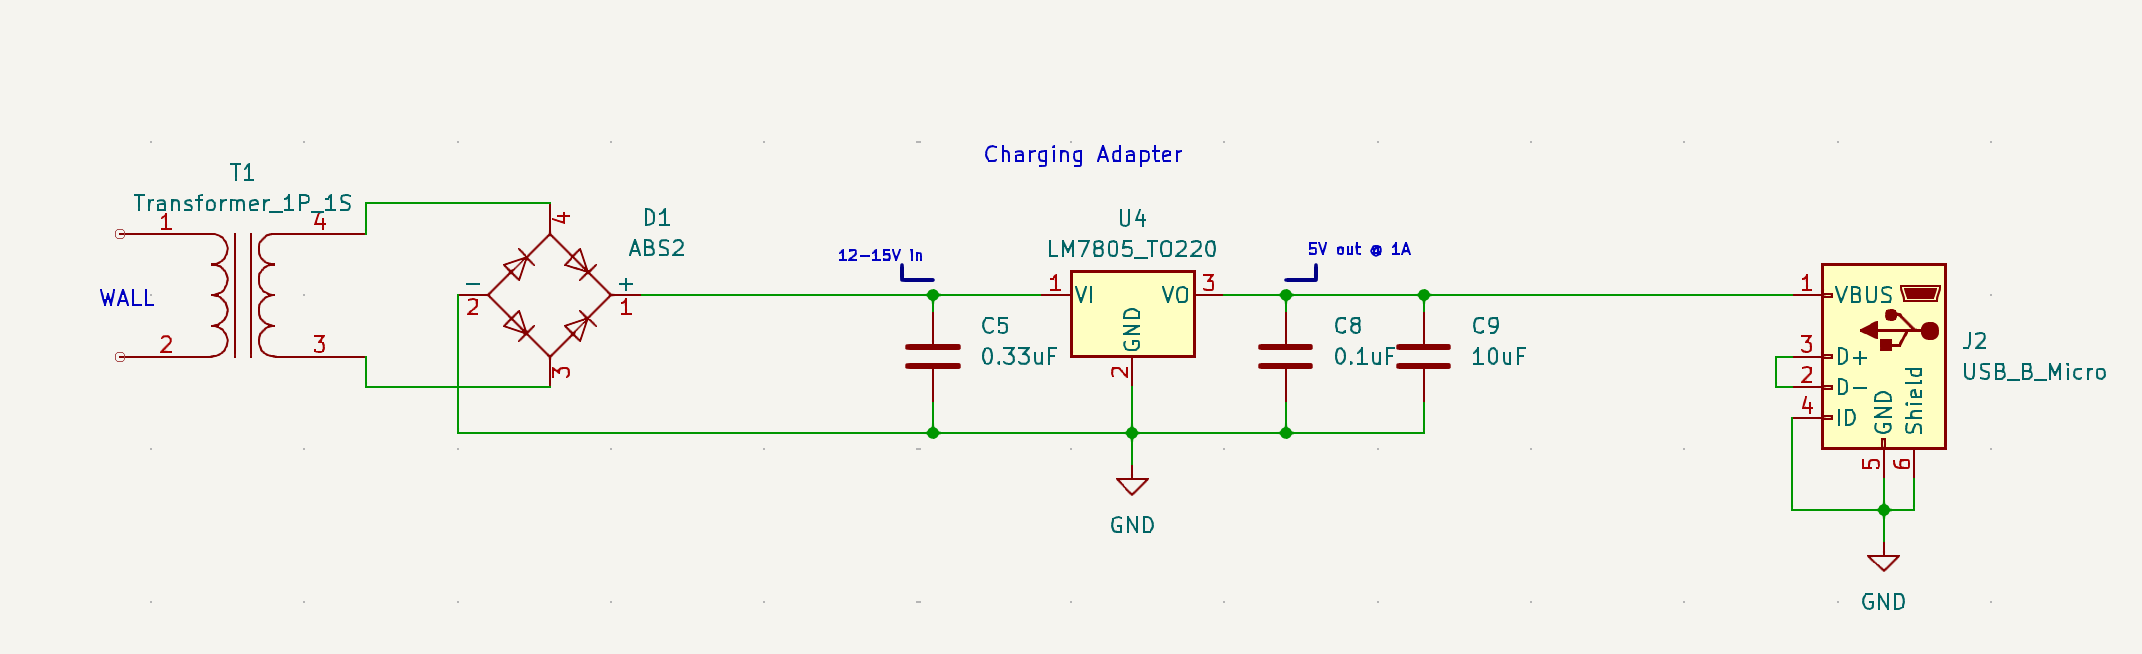
\includegraphics[width=0.7\textwidth]{Adapter.png}
    \caption{Schematic of the Adapter Module}
    \label{fig:adapter_module}
\end{figure}


\section{Charging Module}

The charging module allows the system to operate wirelessly with a LiPo battery.

\begin{itemize}
    \item A USB-C connector feeds power into the module.
    \item The MCP738311/2 LiPo charging IC handles battery charging at a max of 500mA.
    \item PMOS switching circuitry automatically disables battery discharge during external power input.
    \item Once unplugged, battery resumes supplying power.
\end{itemize}

\section{Booster Module}

To drive the ESP32-CAM at stable voltage levels, we use the MT3608 booster module.

\begin{itemize}
    \item It boosts the 3.7V LiPo battery to 5.1V with max output current of 1.5A.
    \item The battery used is rated at 1000mAh with a discharge capacity of 2C.
    \item This makes the module portable and supports moderate current draw without brownouts.
\end{itemize}

The system is designed to switch seamlessly between charging and discharging modes, ensuring stable operation throughout usage cycles.

\begin{figure}[H]
    \centering
    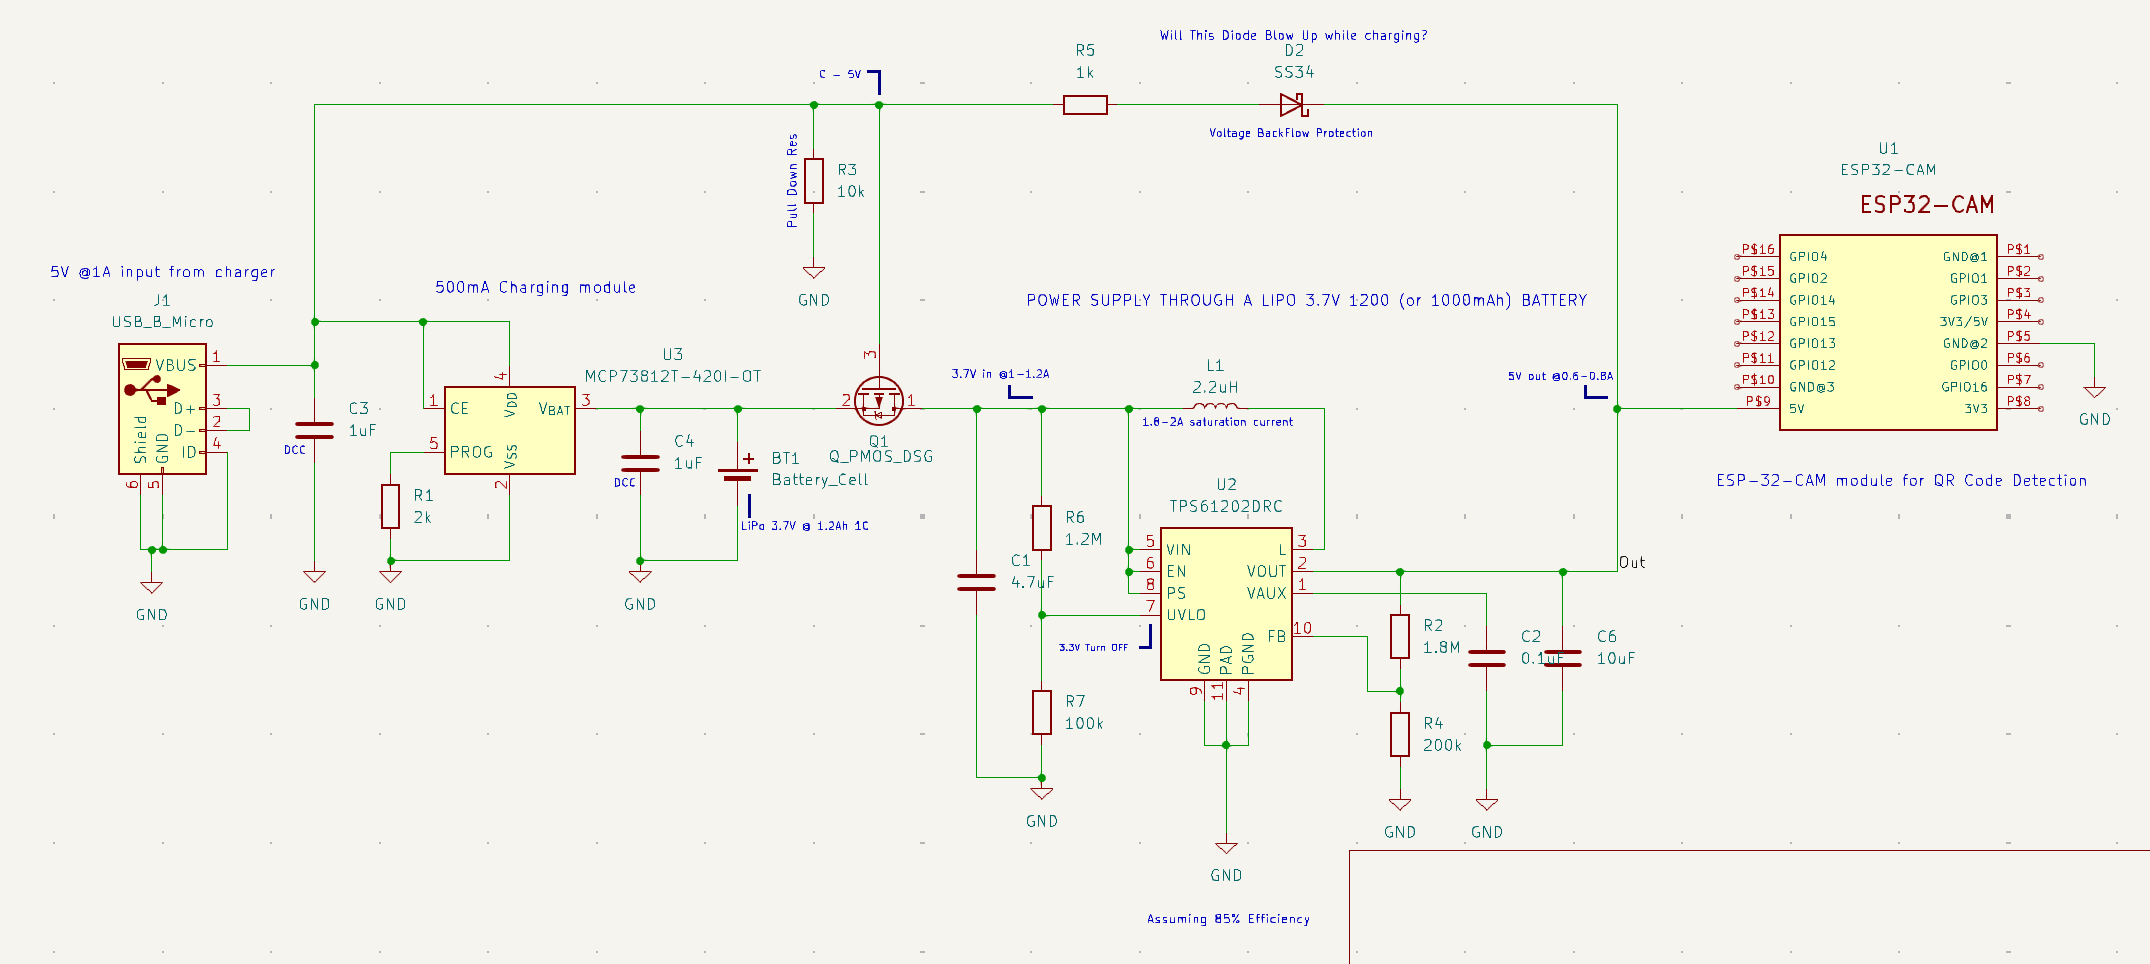
\includegraphics[width=0.7\textwidth]{MultiplexCHD.png}
    \caption{Schematic of the Multiplexed Charger and Booster Module}
    \label{fig:adapter_module}
\end{figure}

\section{ESP32 Cam Scanner Modue}
This is the Last module which uses the ESP32-CAM to Detect QR codes and take photos and send it to the user!

\begin{itemize}
    \item Camera Module - \textbf{MODULE NAME}
    \item Supply Pin Used was 5V one, as evident from the above module.
    \item The ESP Send the image and QR data to the user via a telegram bot for ease of access and minimal setup!
\end{itemize}
